\documentclass[a4paper,12pt]{article}
\usepackage[utf8]{inputenc}
\usepackage{graphicx}
\usepackage{hyperref}
\usepackage{listings}
\usepackage{amsmath}
\usepackage{amssymb} 
\usepackage{xcolor} 


\title{GlusterFS Distributed File System Report}
\author{Group 14}
\date{\today}

\begin{document}

\maketitle

\begin{center}
    \Large \textbf{Group 14 Members:}\\[1cm]
    \large Phan Dang Nhan-BI12-336\\[0.5cm]
    \large Le Ba Hai Long-22BI13261\\[0.5cm]
    \large Do Ba Hoang Minh-22BI13278\\[0.5cm]
    \large Tran Duc Manh-22BI13274\\[0.5cm]
    \large Do Huu Nam-BI12-305 5\\[0.5cm]
    \large Truong Xuan Hieu-22BI13163\\[0.5cm]
    \large Nguyen Hoang Tuan Anh-22BI13023\\[1cm]
\end{center}



\tableofcontents

\newpage

\section{Abstract}
Our project is to create a system that operates similar to GlutterFS (GlutterFS clone) based on the knowledge of distributed system. The system will focus on exploiting the main features of the GlutterFS system such as allowing management, retrieval, and storage of files in a distributed system. In addition, the system provides a basic interface in Visual Studio Code for users to easily interact with the system.
\section{Introduction}
\subsection{Overview}
The purpose of this project is to implement a lightweight distributed filesystem inspired by GlusterFS. This system enables the storage, retrieval, and management of files across multiple nodes while maintaining fault tolerance and scalability. It is designed to provide a simple interface for users to interact with distributed storage resources.

\subsection{Distributed system  }
A distributed filesystem allows data to be stored on multiple servers while appearing as a single cohesive storage unit for the end user. This architecture improves scalability, fault tolerance, and data accessibility.
\subsection{GlutterFS}
\textbf{Overall}
GlusterFS is an open source distributed file system that aggregates storage resources from multiple servers into a unified namespace. It is designed for high scalability, providing features like file replication, striping, and self-healing capabilities. 

A basic GlutterFS system will consist of main components such as Brick, Volume, Storage and Client. Each component will play a different role in the system.



\textbf{Disadvantage of GlutterFS}
 \begin{itemize}
     \item\textbf{Performance}
     \begin{itemize}
         \item Low I/O throughput: GlusterFS is not optimized for applications with heavy random I/O workloads
         \item Network overhead: Synchronizing data over the network can create bottlenecks, especially in environments with multiple clients.
     \end{itemize}
     \item\textbf{Complexity}
     \begin{itemize}
         \item Configuration and management: Setting up and configuring GlusterFS requires in-depth knowledge, making system administration challenging
         \item Scalability issues: While designed for scalability, managing a large number of nodes can become increasingly complex.
         \item Inspired by these principles, this project implements a simplified version to demonstrate core functionalities such as file distribution, storage management, and fault detection
     \end{itemize}
 \end{itemize}


\begin{figure}[htbp]
    \centering
    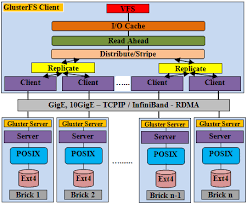
\includegraphics[width=0.5\linewidth]{image\GlutterFS_System.png}
    \caption{GlutterFS system}
    \label{fig:enter-glutterfs}
\end{figure}



\subsection{Objective}
\begin{itemize}
    \item Create a distributed system based on the GlutterFS system (GlutterFS clone)
    \item Create a lighter system, suitable for a wider range of users
    \item Create a basic User interface, making it easy for users to manipulate the system
    
\end{itemize}




\section{Architecture}
\subsection{System diagram}

\begin{figure}[htpd]
    \centering
    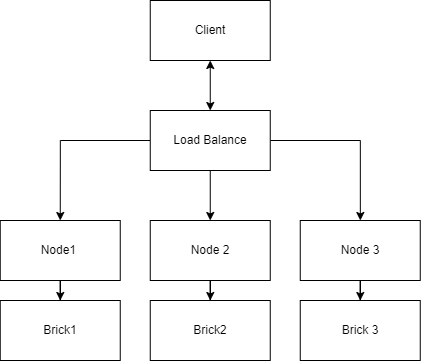
\includegraphics[width=0.5\linewidth]{image\System_Diagram.png}
    \caption{Enter Caption}
    \label{fig:enter-label}
\end{figure}

  Overview of our system, our system focuses on retaining the main components of the normal GlutterFS structure. The system will include Client, Load Balance (acting as Volume), Node and Brick.

Our system is lighter and simpler than a normal Glutter system. By using the commands

\textbf{Explaination}
\begin{itemize}
    \item\textbf{Client}
    \begin{itemize}
        \item Acts as the user-facing interface
        \item Sends commands like store, retrieve and add more node to the system
        \item Interacts with the load balancer to direct requests to appropriate nodes
    \end{itemize}

    \item\textbf{Load Balancer}
    \begin{itemize}
        \item Serves as an intermediary between the client and the nodes.
        \item Distributes requests intelligently to ensure even workload distribution across nodes
        \item Handles node selection based on availability and possibly load metrics.
    \end{itemize}
    
    \item\textbf{Nodes}
    \begin{itemize}
        \item Represent the storage units of the system.
        \item Each node is assigned a unique ID and port (e.g., Node 1 on port 5001)
        \item Perform file storage, retrieval, and heartbeat communication with other nodes for fault detection.
    \end{itemize}
\end{itemize}




\subsection{Sequence Diagram}
Our entire system works as follows. Users will create nodes that act as servers. Each node is capable of storing files, retrieving them, and communicating with other nodes to detect errors. Each node will run on a separate port. In our case, we create 3 nodes with 3 separate ports 5001, 5002, 5003

After creating a node, the user will launch a Client to interact with the system. After the user interacts with the system, the system will send the client's requests to the load balancer. The load balancer will send the information to the appropriate node. The appropriate nodes receive the information and return the results to the load balancer
 \begin{itemize}
     \item \textbf{Store Function}
         \begin{figure}[htbp]
         \centering
         \includegraphics[width=0.75\linewidth]{image\StoreFunction.png}
         \caption{StoreFunction}
         \label{fig:enter-store}
     \end{figure}

     
     The StoreFunction receives a request from the client to store the file. After the client issues a store command, the request is forwarded to the load balancer, which determines the most suitable node to store the file.
     Upon receiving the request, the selected node processes the data and writes the data to that node. After the file is successfully stored, the node sends an acknowledgement back to the load balancer, which then forwards the information to the client, informing the user that the file has been stored.



 
     \item \textbf{Retrieve Function} 
         \begin{figure}
         \centering
         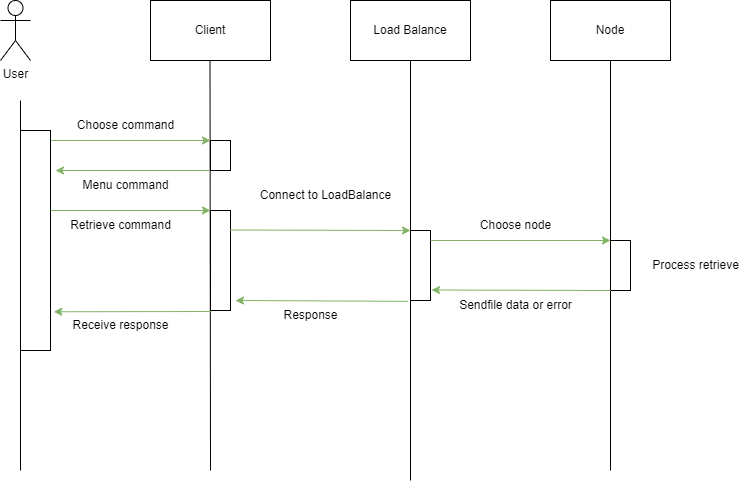
\includegraphics[width=0.5\linewidth]{image\Retrieve Function.drawio.png}
         \caption{Retrieve Function}
         \label{fig:enter- retrieve}
     \end{figure}

     
     When a client makes a request to retrieve a file, the load balancer ensures that the client receives the file from the correct node. The load balancer determines which node contains the requested file and forwards the request accordingly. The node sends the file back to the load balancer. From there, the data is passed back to the client, completing the retrieval process.
     
     
     \item \textbf{Heartbeat Function}
     \begin{figure}[htbp]
         \centering
         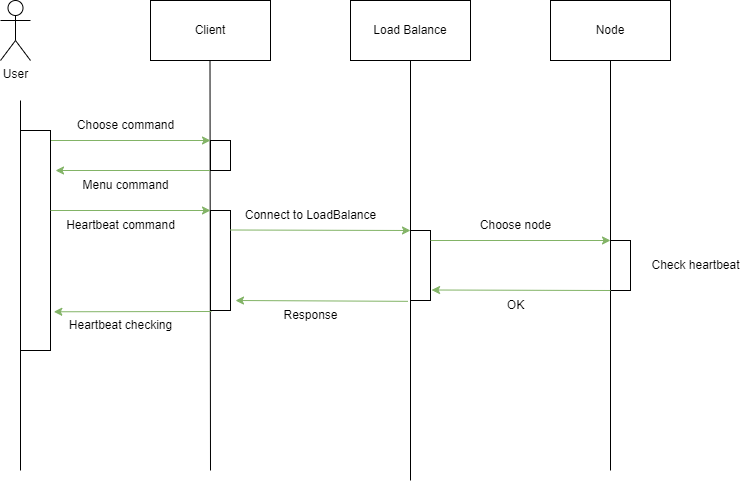
\includegraphics[width=0.5\linewidth]{image\Heartbeat Function.drawio.png}
         \caption{Heartbeat Function}
         \label{fig:enter-heartbeat}
     \end{figure}

     Each node in the network periodically sends a “heartbeat” signal to a central management unit, typically a load balancer or a dedicated monitoring service. This signal indicates that the node is still functioning. If a node fails to send a heartbeat within a specified time frame, the system marks the node as potentially failing. This failure detection mechanism allows the system to respond quickly to failing nodes by rerouting requests to healthy nodes or initiating corrective actions such as rebooting the failed node or reallocating its workload.
     
 \end{itemize}


\section{Methodology}

\begin{itemize}
    \item System Design: We started by designing the system architecture based on the GlusterFS model, focusing on the main components such as Client, Load Balancer, Nodes and Bricks. This design aims to create a simpler and lighter version of the GlusterFS system.
    \item Node Management: Nodes are designed to handle file storage and retrieval, and communicate with each other to detect failures. We ensure that each node is independent and can operate with minimal intervention.
    \item Client User Interface: A simple client interface is created to send commands to the system, such as file storage, retrieval and node management. This interface is designed to be easy to use and integrate smoothly with the rest of the system.
         \begin{figure}[htbp]
        \centering
        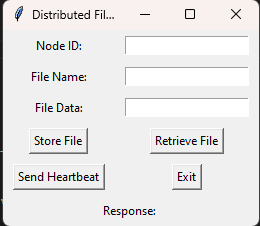
\includegraphics[width=0.5\linewidth]{image\Interface.png}
        \caption{Interface}
        \label{fig:enter-label}
    \end{figure}
        \item 
Load Balancer: The Load Balancer is designed to intelligently distribute requests from clients to the appropriate node, ensuring an even distribution of workload across nodes. This component is critical for fault tolerance and scalability of the system.
    \item File storage and retrieval: We have implemented core functionality for storing and retrieving files from nodes. Each file is stored on a single node, but the retrieval process is designed to ensure that clients can always access their files reliably.
\end{itemize}



\section{Limitations and Future Improvements}
 \subsection{Limitations}
 \begin{itemize}
     \item Centralized client interface introduces a single point of failure
     \item No encryption for file transfer
     \item Lack of replication for high availability.
 \end{itemize}
\subsection{Future Improvement}
\begin{itemize}
    \item Cloud storage backends.
    \item Big data analytics frameworks such as Hadoop and Spark.
    \item Virtualization environments for storing VM images.
\end{itemize}

\section{Conclusion}
GlusterFS exemplifies the modern approach to distributed file systems, offering a balance of scalability, reliability, and cost-effectiveness. Its ability to function seamlessly across commodity hardware, combined with its flexibility in handling diverse workloads, makes it an indispensable tool in today’s data-driven world. By providing features such as distributed storage, self-healing, and high availability, GlusterFS addresses the critical challenges of managing large-scale storage systems, solidifying its position as a robust solution for enterprises and developers alike.

\section*{References}
\begin{itemize}
    \item GlusterFS Documentation: \url{https://docs.gluster.org/}
    \item Relevant research papers and case studies.
\end{itemize}

\end{document}
